\documentclass[a4paper, 12pt]{article}

\usepackage[utf8]{inputenc}
\usepackage[portuguese]{babel}
\usepackage[T1]{fontenc}
\usepackage{graphicx}

\usepackage{amsmath, amsfonts, amssymb}
\usepackage{siunitx}
\usepackage{hyperref}

\newcommand{\tbf}[1]{\textbf{#1}}

\usepackage[top=2cm, left=2cm, bottom=2cm, right=2cm]{geometry}

\usepackage{fontspec}
\setmainfont{Arial}

\begin{document}
	\begin{itemize}
		\item\textbf{Nome: Renan da Silva Guedes}
		\item\textbf{RA: 223979}
	\end{itemize}
	
	\begin{center}
		\begin{large}
			\uppercase{Estudo dirigido 4}
		\end{large}
	\end{center}
	
	\begin{enumerate}
		\item\tbf{Explique a Lei de Stefan - Boltzmann.}
		
		Ela enuncia que todo o corpo com temperatura acima de \SI{0}{\kelvin} emite energia radioativa, e esta lei diz que a \textit{densidade de fluxo} de energia emitida (E, em $\SI{}{\watt/\,\meter^{2}}$) é proporcional  à quarta potência de sua temperatura absoluta (T, em \SI{}{\kelvin}), de acordo com a equação $\textrm{E}=\epsilon\,\sigma\,\textrm{T}^{4}$, onde $\epsilon$ é o poder emissivo do corpo, $\sigma$ é a constante de Stefan - Boltzmann ($=\SI{5.67e-8}{\watt\meter^{-2}\kelvin^{-4}}$)
		
		\item\tbf{Explique a Lei de Wien.}
		
		Esta lei estabelece que o produto da temperatura absoluta (T, em \SI{}{\kelvin}), do objeto, pelo comprimento de onda ($\lambda_{\textit{máx}}$, em \SI{}{\nano\meter}) de máxima emissão energética, do próprio objeto, é constante, ou seja $\textrm{T}\,\lambda_{\textit{máx}}=\textrm{constante}=\SI{2.898e6}{\nano\meter\kelvin}$. Esta lei é fundamental para o entendimento do balanço energético na superfície da Terra
		
		\item\tbf{Como a latitude influencia o fotoperíodo de um local?}
		
		O fotoperíodo está vinculado aos intervalos de luz os quais a planta é submetida. Dessa forma, a variação da latitude influência na disponibilidade de luz em determinados pontos do planeta. Regiões mais próxima dos trópicos tendem a receber luz com menor intensidade e tempo de exposição quando comparadas ao equador, sendo essas grandezas inversamente proporcionais a latitude local.
		
		\item\tbf{Quais os principais aparelhos que medem radiação solar?}
		
		Os principais aparelhos utilizados são: Os solarímetros, piranômetros, pireliômetros, radiômetros e actinógrafos.
		
		\item\tbf{Você está trabalhando em uma propriedade agrícola que não há aparelhos para medição de radiação solar. Explique como você poderia obtê-la.}
		
		Por meio das relações trigonométricas é possível determinar a radiação solar na superfície terrestre em determinado instante. Esse método é funcional tendo em vista que o ângulo zenital ($\textrm{Z}_{\text{h}}$) varia de acordo com a latitude ($\Phi$), do horário do dia (h), e da declinação solar ($\delta$). Dessa forma, com base na estação do ano e nas grandezas referidas é possível determinar os valores para cada época do ano e geolocalização no globo, levando em consideração a incidência normal dos raios solares.
		
		\item\tbf{Você foi contratado para assessorar uma fazenda no oeste do Estado de São Paulo (Lat. $21^{\circ}05'\,\textrm{S}$; Long. $51^{\circ}00'\,\textrm{W}$ e Alt. \SI{680}{\meter}), num município onde não existem informações climáticas. O dono da fazenda requisita um projeto de viabilidade do cultivo econômico do pessegueiro. No levantamento bibliográfico você verifica que para se desenvolver bem essa planta necessita de temperatura média mensal inferior a \SI{17}{\celsius} durante pelo menos três meses consecutivos por ano. A cultura é ou não é recomendável para essa região? Qual a importância da previsão de frente fria para agricultura?}
		
		Com base no gráfico extraído do INMET (Instituto Nacional de Meteorologia), para a região do município de Três Lagoas (Lat. -20.7833968, Long. -51.7345538) vê-se que para a época de inverno as temperaturas médias encontram-se acima do limite para o cultivo econômico do pessegueiro, dessa forma, seria inviável lançar mão de recursos para o implemento com base no gráfico abaixo.
		
		\begin{figure}
			\centering
			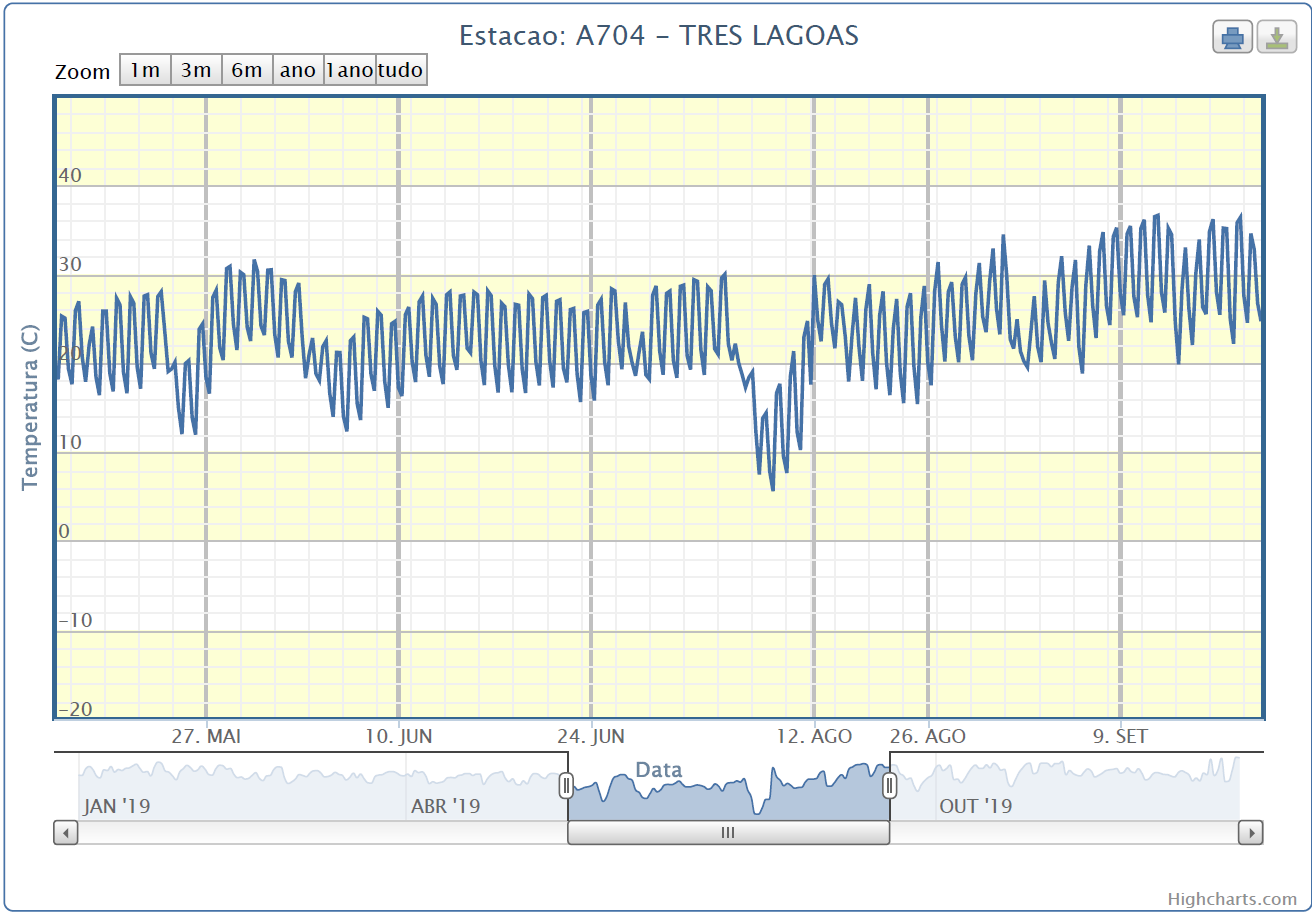
\includegraphics[scale=.35]{images/print}
			\caption{Gráfico extraído do INMET com dados de 27 de maio a 9 de setembro para o município de Três Lagoas em 2019. Disponível em:  \href{http://www.inmet.gov.br/portal/index.php?r=home/page\&page=rede\_estacoes\_auto\_graf}{http://www.inmet.gov.br/portal/index.php?r=home/page\&page=rede\_estacoes\_auto\_graf}}
		\end{figure}
		
		\item\tbf{Você foi requisitado para a instalação de um posto agrometeorológico numa propriedade agrícola. Em que condições você recomendaria a instalação dos termômetros para medir temperatura do ar e do solo?}
		
		Para medir a temperatura do ar é recomendável a instalação de termômetros de 1.5 a \SI{2}{\meter} acima da superfície. Para aferir a temperatura do solo recomenda-se a instalação dos termômetros num solo coberto por vegetação de modo a evitar grandes variações no gradiente de temperatura. Dessa forma, por meio de uma estação automática, pode ser feita a coleta em múltiplos instantes da temperatura visando a obtenção da média diária ou mensal para o tipo de solo presente na propriedade.
		
		\item\tbf{Explique a relação da umidade relativa do ar com a temperatura.}
		
		É possível concluir que a umidade relativa é inversamente proporcional à amplitude térmica num intervalo analisado. Ou seja, quanto maior a quantidade de água na forma de vapor no ambiente haverá maior dificuldade para a temperatura variar.
			
		\item\tbf{Quais os principais aparelhos que medem a umidade relativa? Escolha um e explique seu funcionamento.}
		
		Os principais aparelhos são: O psicrômetro, higrógrafo de cabelo e os sensores capacitivos.
		
		Os sensores capacitivos baseiam-se na variação da capacitância num filme de polímero que absorve o vapor d'água. Dessa forma a partir desta variação de capacitância num circuito ativo, com o aporte de um sensor de temperatura é possível executar as medidas. É recomendável fazer calibragens periódicas e limpeza, principalmente em períodos muito secos.
		
		\item\tbf{O que é ponto de orvalho?}
		
		O ponto de orvalho é definido como a temperatura na qual uma parcela de ar atinge a saturação apenas por resfriamento.
		
		\item\tbf{Explique chuva Frontal, orográfica e convectiva.}
		
		A chuva frontal é proveniente do encontro de massas de ar frio e quente. Dessa forma, a massa de ar quente e úmido tende a elevar-se resfriando-se adiabaticamente, nessa subida forçada é ocasionada a condensação.
		
		As chuvas convectivas são  decorrentes do resfriamento adiabático de correntes convectivas (térmicas), produzindo nuvens de grande desenvolvimento vertical e chuvas de forte intensidade porém, de curta duração.
		
		Por fim, as orográficas ocorrem comumente em regiões de relvo mais montanhoso, ocasionadas pelo resfriamento do ar úmido ao elevar sua altitude. Dessa forma, há uma mescla entre nuvens do tipo cumuliformes e estratiformes caracterizando chuvas contrastantes no relevo denominadas \textit{Sombras de chuva}.
		
		\item\tbf{Qual o aparelho que mede chuva? O que significa dizer que chovem \SI{10}{\milli\meter} em um dia?}
		
		O aparelho comumente utilizado para medição da chuva é o pluviômetro; Ao dizer que choveu \SI{10}{\milli\meter} é feita uma referência à altura pluviométrica, na qual é expresso o volume de água acumulada por metro quadrado. Dessa forma, para os \SI{10}{\milli\meter} referidos significaria um acúmulo de 10 litros de água por metro quadrado de terreno.
		
		\item\tbf{Uma cultura de milho foi afetada por um forte vendaval que provocou o acamamento das plantas, inviabilizando a colheita mecânica. A cultura estava segurada, porém o Banco só pagará o seguro se a rajada de vento tiver sido superior a \SI{80}{\kilo\meter/\hour}. No laudo fornecido a velocidade foi de \SI{28.5}{\meter/\second}. Será que o prejuízo será coberto pela seguradora? Explique.}
		
		O prejuízo será coberto pela seguradora, pois o laudo forneceu uma velocidade de $\SI{28.5}{\meter/\second}=\SI{102.6}{\kilo\meter/\hour}$, ultrapassando em \SI{20.6}{\kilo\meter/\hour} do valor estabelecido para cobrimento dos danos à cultura.
	\end{enumerate}
\end{document}